\chapter{Aprendizaje reforzado}

\section{Or\'igenes y descripci\'on}

El Aprendizaje Reforzado se basa en la psicolog\'ia conductista: un \textit{agente} busca ser recompensado con un premio, el cual obtiene cuando realiza una secuencia de \textit{acciones} que lo llevan a concluir una tarea exitosamente. Adem\'as, para maximizar la cantidad de \textit{recompensa} que recibe (o, alternativamente, minimizar el tiempo que espera entre un premio y el siguiente) comienza a optimizar su pol\'itica (\textit{$\pi$}) para llegar a la meta satisfactoriamente. As\'i, tal agente \textit{aprende} estrategias y va \textit{reforzando} el aprendizaje de tales estrategias que maximicen sus recompensas. Una explicaci\'on mucho m\'as profunda de las bases e historia del aprendizaje reforzado, as\'i como la mayor parte de las definiciones mencionadas en este cap\'itulo, pueden ser encontradas en \citet{Sutton}.\\

\subsection{Terminolog\'ia com\'un}

Existen conceptos utilizados en pr\'acticamente la totalidad de los algoritmos de aprendizaje reforzado, independientemente de las particularidades que presenten. A continuaci\'on se presenta una lista, basada en la recopilaci\'on no exhaustiva de ellos de \citet{rlexplained}, pero que cubre los t\'erminos utilizados en este trabajo.

\begin{enumerate}
    \item Agente: es la entidad que aprender\'a durante el proceso. Por ejemplo, puede ser un rat\'on rob\'otico aprendiendo a llegar al queso en el laberinto; o un jugador virtual aprendiendo a superar todos los niveles de un videojuego.
    \item Estado: describe la situaci\'on en la cual se encuentra el sistema. Por ejemplo, para el rat\'on rob\'otico, el estado es la casilla en la que se encuentra. El estado puede tener tantas dimensiones como sea necesario: por ejemplo, el estado de un coche autodirigido ser\'ia descrito por su posici\'on, velocidad, objetos en su radar e incluso cantidad de gasolina en el tanque.
    \item Mundo: se refiere la totalidad de los posibles estados.
    \item Acci\'on: es lo que un agente puede hacer en cada estado. Generalmente, el conjunto de acciones que puede tomar un agente en un estado determinado es finito, aunque el conjunto de acciones que tome durante todo el tiempo pueda tener combinaciones que se aproximen al infinito. Por ejemplo, para el rat\'on rob\'otico, sus acciones son realizar un movimiento hacia adelante, atr'as, derecha o izquierda.
    \item Recompensa: cuando un agente toma una acci\'on en un estado, recibe una recompensa. Es muy importante notar que la recompensa puede tomar muchas formas: es posible que sea solamente la meta \'ultima, en vez de existir despu\'es de cada acci\'on (como el queso para el rat\'on). La recompensa tambi\'en puede ser negativa, equivalente a un castigo, lo cual causa que el agente aprenda a evitar las acciones que lo llevan a ella.
    \item Pol\'itica (\textit{policy}) es una funci\'on que toma como argumento un estado $s$ y devuelve una acci\'on $a$; equivalente a la estrategia del agente. La meta del aprendizaje reforzado es encontrar la pol\'itica \'optima. Generalmente se le representa como $\pi(s)\rightarrow a$.
\end{enumerate}

La relaci\'on entre estos conceptos se puede consultar en la Figura \ref{rl_concepts}, popularizada por \citet{Sutton}.\\

\begin{figure}[ht]
\caption{Interacci\'on de los conceptos en Aprendizaje Reforzado}
\label{rl_concepts}
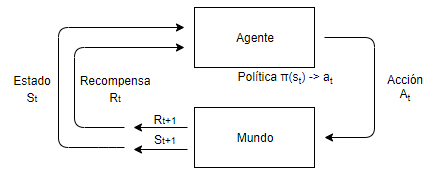
\includegraphics[width=10cm]{tesis_tex/figs/rl_concepts.PNG}
\centering
\end{figure}

Una vez que tenemos asignados estos elementos, resulta relativamente simple explicar el problema, pero no as\'i la implementaci\'on. Por ejemplo, rat\'on solamente recibir\'a la recompensa despu\'es de un movimiento espec\'ifico que lo lleve a la casilla en la que se encuentra el queso; todos los dem\'as movimientos son solamente un medio para acercarse. El aprendizaje reforzado resuelve esta situaci\'on asign\'andole valor a las recompensas a largo plazo en vez de solamente a las inmediatas. Esto quiere decir que si planteamos el objetivo del aprendizaje como llegar al queso, el rat\'on no podr\'a decidir si es mejor un camino m\'as r\'apido o uno en el que dio vueltas sin sentido en un mismo lugar, siempre que en un tiempo finito haya llegado al final. Sin embargo, si descontamos el valor del queso por cada casilla extra que le toma llegar a \'el, entonces buscar\'a el camino m\'as corto, optimizando su secuencia de acciones interactuando con el mundo que lo rodea para descubrir relaciones acci\'on-estado. La representaci\'on matem\'atica de este problema se condensa en la \textit{Ecuaci\'on de Bellman}, la cual ser\'a desarrollada en la siguiente secci\'on, pero de una manera muy simple podr\'ia ser representada como:\\

\textit{Recompensa $=$ Valor cal\'orico del queso $-$}

\hspace{22mm} \textit{Calor\'ias necesarias para moverse una casilla * Total de casillas visitadas}
  
\subsection{La ecuaci\'on de Bellman}  
    
La principal caracter\'istica del agente es que tiene la capacidad de tomar decisiones sobre sus acciones, las cuales son su forma de interactuar con el mundo, llev\'andolo de un estado a otro. El agente no tiene acceso a todas las consecuencias de sus acciones; de hecho, ni siquiera conoce todo el mundo. Adem\'as, como se ver\'a, su percepci\'on es que no existe un retraso en la recompensa.\\

El agente toma una acci\'on en el tiempo $t$, la cual depende del estado $s_t$ del mundo. En $t+1$, el mundo reaccion\'o ya a la interacci\'on del agente con \'el, as\'i que el agente recibe una recompensa $r_{t+1}$ y toma una nueva acci\'on dependiendo del estado $s_{t+1}$ del mundo. Sin embargo, no es \'optimo seleccionar acciones solamente con base en la recompensa $r_{t+1}$, pues la naturaleza temporal del problema lo convierte en un problema a largo plazo, y el agente estar\'ia considerando solamente consecuencias en el corto plazo.\\

As\'i, el agente debe aprender que existe un \textit{retraso} entre cada acci\'on que toma y el premio. Supongamos que, en una cuadr\'icula, el premio se encuentra en la casilla $(x,y)$. El agente solamente puede llegar a esa casilla meta desde las adyacentes, pero si no se encuentra en una de estas, primero debe acercarse a alguna de las casillas adyacentes, por ejemplo $(x-1,y)$. Recursivamente, si no se encuentra en ninguna de estas casillas, debe encontrar un camino que lo lleve ah\'i. Este proceso se conoce como \textit{exploraci\'on}, pues es posible que el agente no reciba ninguna recompensa por sus acciones hasta que encuentre por primera vez la casilla (x,y) en el tiempo $t$ y asigne un valor de recompensa positivo (aunque descontado) a la casilla en la que se encontraba al tiempo $t-1$. As\'i, cuando el agente comienza su exploraci\'on, ir\'a aprendiendo que, lejos de que la recompensa sea inmediata, debe tomar una secuencia de acciones para llegar a ella. Una vez que el agente tiene mejor conocimiento acerca de cu\'ales casillas lo acercan al premio, pasa a una fase llamada \textit{explotaci\'on}, en la cual busca la recompensa m\'as grande entre todas las que conoce. Un agente debe comenzar su aprendizaje puramente en modo exploratorio, y transicionar al modo de explotaci\'on conforme conoce mejor su ambiente.\\

Podemos entonces definir la \textit{funci\'on de valor} asociada a la pol\'itica como el valor esperado de la recompensa al tiempo $t$ dado que el agente se encuentra en el estado $s$. Adem\'as, cada periodo de tiempo se le aplica un factor de descuento $\gamma$ para obtener el valor presente de tal recompensa. De esta definici\'on deriva uno de los conceptos m\'as importantes en el aprendizaje reforzado, la \textit{Ecuaci\'on de Bellman}. A continuaci\'on se explica el desarrollo de esta, obtenido de \citet{Sutton}. \\

La idea b\'asica es que la recompensa total en el tiempo $t$ es que se compone de la recompensa parcial en el tiempo $t+1$ despu\'es de tomar alguna acci\'on; m\'as la recompensa parcial en el tiempo $t+2$, descontada porque existe un retraso y tomando en cuenta que se proviene de un estado $s$ posible si el agente tom\'o la acci\'on que tom\'o en el tiempo $t+1$, y as\'i sucesivamente. Esto se representa con la siguiente ecuaci\'on recurrente:

\vspace{-30pt}
\begin{align*}
R_{t} &= r_{t+1} + \gamma r_{t+2} + \gamma^{2} r_{t+3} + \gamma^{3} r_{t+4} + ... \\
    &= r_{t+1} + \gamma \left( r_{t+2} + \gamma r_{t+3} + \gamma^{2}r_{t+4} + ...  \right)  \\
    &= r_{t+1} + \gamma R_{t+1}
\end{align*}

El valor de un estado $s$ se puede definir como la recompensa esperada dado que el agente empieza en ese estado, y depende de su pol\'itica:

$$
V^{\pi}(s) = E_{\pi}\left\{R_{t}|s_{t} = s\right\} = E_{\pi}\left\{\sum_{k=0}^{\infty}\gamma^{k}r_{t+k+1}|s_{t}=s\right\}.
$$

\subsection{El m\'etodo $\epsilon$\textit{-greedy}}

Cuando una persona se muda a una nueva ciudad, es posible que quiera encontrar su nuevo restaurante favorito. Al principio experimentar\'a en muchos restaurantes, probar\'a comida nueva, e ir\'a descubriendo el mundo y acumulando aprendizaje. Despu\'es de alg\'un tiempo, esta persona ya tendr\'a una idea bastante robusta de cu\'al(es) restaurante(s) le gusta(n), as\'i que m\'as bien explotar\'a este conocimiento e ir\'a ah\'i m\'as seguido. Sin embargo, si mantiene sus opciones abiertas y de vez en cuando visita un restaurante nuevo, podr\'ia encontrar su nuevo favorito.\\

El m\'etodo $\epsilon$\textit{-greedy} es una manera de  que el agente ajuste su comportamiento mientras transcurre el tiempo: al principio debe \textit{explorar} para conocer la mayor cantidad de consecuencias a sus acciones posibles, pero m\'as adelante debe \textit{explotar} el conocimiento de cu\'ales acciones le han reportado buenas recompensas y tomar esas decisiones m\'as seguido. \\

Definamos $p_r{t}$ y $p_t{t}$ como las probabilidades al tiempo $t$ de exploraci\'on y explotaci\'on, respectivamente. Entonces:

\vspace{-30pt}
\begin{align*}
p_r{t} &= 1 - \epsilon(t) \\,
p_t{t} &= 1 - p_r{t} \quad \quad \forall t.
\end{align*}

A esta estrategia de exploraci\'on se le llama $\epsilon-greedy$ porque el agente es codicioso (en ingl\'es, \textit{greedy}) al querer siempre buscar la m\'axima recompensa posible, pero limitado por la funci\'on $\epsilon$. Tal funci\'on suele ser implementada como decreciente de forma lineal para el aprendizaje, de tal forma que mientras pasa el tiempo, el agente escoge las acciones conocidas que le reportan mayor utilidad m\'as seguido. De esta manera se asegura que siempre existe una probabilidad positiva de explorar.\\

\subsection{Los MDP (procesos de decisi\'on de Markov)}

Un algoritmo de aprendizaje reforzado que cumple con la propiedad de Markov se llama Proceso de Decisi\'on de Markov (MDP, por sus siglas en ingl\'es). La propiedad de Markov a grandes rasgos, dice que el futuro solamente depende del estado obtenido con las acciones inmediatamente anteriores, no del pasado que haya transcurrido previamente. En t\'erminos formales (\cite{Sutton}), si se supone que existen un n\'umero finito de estados y recompensas \footnote{Si el supuesto de finitez para los estados de recompensas es removido, el argumento debe ser extendido a integrales y densidades de probabilidades en lugar de sumas y probabilidades.}, entonces se puede considerar c\'omo un mundo responder\'ia en el tiempo $t+1$ a la acci\'on tomada en el tiempo $t$. Esto se describe con la distribuci\'on conjunta de probabilidad:\\

\vspace{-30pt}
\begin{align*}
P\{S_{t+1} = s', R_{t+1} = r \quad | \quad S_{0}, A_{0}, R_{1}, ... , S_{t-1}, A_{t-1}, R_{t}, S_{t}, A_{t} \},
\end{align*}

\noindent para todos las recompensas $r$, estados $s'$ y todos los valores posibles de los eventos pasados: $_{0}, A_{0}, R_{1}, ... , S_{t-1}, A_{t-1}, R_{t}, S_{t}, A_{t}$. La propiedad de Markov indica que la respuesta del mundo en el tiempo $t+1$ depende solamente del estado y acciones en el tiempo $t$, es decir:

\vspace{-30pt}
\begin{align*}
p\left(s', r \quad | \quad s,a \right) = P\{S_{t+1} = s', R_{t+1} = r \quad | \quad S_{t} = s, A_{t} =a\},
\end{align*}

\noindent para todos las recompensas $r$, estados $s'$ y acciones $a$. Si el mundo tiene la propiedad de Markov, entonces es posible calcular la recompensa esperada dado un estado actual y una acci\'on.\\

Formalmente, un Proceso de Decisi\'on de Markov es una tupla $(X,U,f,\rho)$ en donde $X$ es el conjunto finito de estados, $U$ es el conjunto finito de acciones de un agente en un estado, $f:X \times U \times X\rightarrow[0,1]$ es la funci\'on de probabilidad de transici\'on de estado, y $\rho:X \times U \times X\rightarrow\mathbb{R}$ es la funci\'on de recompensa. Es evidente que las pol\'iticas anteriores no juegan un rol, solamente el estado en el que se encuentra el agente.\\

Cuando el conjunto de acciones (o la pol\'itica) a tomar es dif\'icil de aprender porque no existen ejemplos, o el mundo/conjunto de acciones/conjunto de consecuencias es demasiado grande (e.g. infinito), es apropiado utilizar Aprendizaje de M\'aquina Reforzado en lugar de Aprendizaje de M\'aquina regular (i.e. modelos supervisados o no supervisados). Gracias a que el agente va descubriendo y acerc\'andose a una pol\'itica \'optima, no es estrictamente necesario que explore todas las acciones posibles. \\

En este trabajo se aplicar\'an dos algoritmos sumamente conocidos y aplicados en un sinf\'in de \'ambitos: \textit{Policy Iteration} y \textit{Q-learning}, y compararemos su rendimiento al aplicarlos al problema de la distribuci\'on de cerveza.

\section{\textit{Policy Iteration}}

En este algoritmo, se empieza con una pol\'itica aleatoria, se encuentra su valor y se realiza un paso que encuentra una pol\'itica nueva (mejor) basado en la anterior. Bajo el supuesto de que los agentes tienen una cantidad finita de acciones en cada estado, existen una cantidad finita de posibles pol\'iticas y es razonable esperar convergencia en un algoritmo de b\'usqueda. De cierta manera, dado un tiempo suficientemente grande y cardinalidad finita de las acciones a tomar en cada estado por cada agente, \textit{policy iteration} encuentra una pol\'itica \'optima. En general, el algoritmo parece terminar en tiempo exponencial o pseudopolinomial, pero el m\'aximo tiempo posible es todav\'ia un tema abierto de investigaci\'on.\\

Recordemos que en cada tiempo $t$, cada agente puede tomar una acci\'on $a$ y recibe una recompensa $r$. De manera general se puede suponer que debido a esto, el proceso de aprendizaje se comporta como un proceso de decisi\'on Markov (MDP). As\'i, de manera iterativa se puede asignar una pol\'itica $\pi$ a cada agente (es importante recordar que una pol\'itica es el conjunto de acciones $a_t$ a tomar en cada estado $e_t$), evaluar su desempe\~no por medio de la recompensa final que representa para el agente, y avanzar a la siguiente iteraci\'on en la cual se intentar\'a mejorar la mejor pol\'itica hist\'orica.\\

Esto quiere decir que, tomando una pol\'itica base $\pi_0$, se puede encontrar una pol\'itica $\pi_1$ que otorga una recompensa igual o mayor (i.e. $V^{\pi_0}(s)<V^{\pi_1}(s) \forall s \in S$). En alg\'un momento, el algoritmo llega a una pol\'itica $\pi_{*}$ que no puede ser mejorada, la cual es declarada la pol\'itica \'optima.\\


Se puede representar este proceso como:

$$
\pi_0 \overset{E}{\rightarrow} V^{\pi_{0}} \overset{I}{\rightarrow}
\pi_1 \overset{E}{\rightarrow} V^{\pi_{1}} \overset{I}{\rightarrow}
\pi_2 \overset{E}{\rightarrow} 
...
\overset{I}{\rightarrow} \pi_{*} \overset{E}{\rightarrow} V^{\pi_{*}}
$$

En donde $\overset{E}{\rightarrow}$ significa que una pol\'itica se \textit{eval\'ua}, y $\overset{I}{\rightarrow}$ significa que se mejora (por \textit{improvement}, en ingl\'es). \\

Las ecuaciones que representan el algoritmo se presentan a continuaci\'on como son descritas por \citet{Frazzoli}. Para encontrar el valor de cada estado bajo la pol\'itica $\pi$:

$$
V(s) = \sum_{s' \in S}^{ } T(s, \pi(s), s')[R(s, \pi(s), s') + \gamma V(s')] \quad \forall s \in S
$$

Para mejorar la pol\'itica, se aplica para cada $s \in S$:

$$
\pi(s) \leftarrow \max_a \sum_{s' \in S}^{ }T(s,a,s')[R(s,a,s') + \gamma V(s')]
$$

iterando ambos pasos hasta que converja a una $\pi_*$.\\

El modelo desarrollado en este trabajo ser\'a implementado como un algoritmo de \textit{policy iteration}. Algunas partes relevantes del c\'odigo se pueden consultar en el cap\'itulo  \ref{ch:resultados}.\\

Existe un algoritmo similar llamado \textit{value iteration}, el cual itera sobre la funci\'on de valor e infiere la pol\'itica relacionada al valor \'optimo obtenido al final, en lugar de iterar sobre la pol\'itica y evaluar el valor. Se suele preferir el algoritmo de \textit{policy iteration} sobre \textit{value iteration}, pues converge m\'as r\'apidamente (en t\'erminos de iteraciones necesarias), presumiblemente porque la funci\'on de valor cambia muy poco de una pol\'itica a otra. Adem\'as, dado que se itera sobre la pol\'itica anterior y se busca una mejor, el algoritmo converge r\'apidamente y cada paso asegura una mejora. Se puede consultar m\'as acerca del algoritmo \textit{value iteration} y de la programaci\'on y convergencia de ambos en \citet{Sutton}.

\section{Q-Learning}

Uno de los algoritmos m\'as populares de aprendizaje es \textit{Q-learning}. Obtiene este nombre por la \textit{funci\'on Q}, que indica el valor descontado de la recompensa asociado a una acci\'on en un estado determinado. La principal ventaja de este tipo de aprendizaje es que no est\'a basado en un modelo, es decir, que se conoce una cantidad m\'inima de detalles acerca del mundo y su funcionamiento, y el agente aprende con base en su experiencia al interactuar. Esta libertad permite, por ejemplo, relajar el supuesto del proceso comport\'andose como un proceso de Markov.

\subsection{Conceptos}

Recordemos la ecuaci\'on de valor de un estado, basada en la ecuaci\'on de Bellman, que fue desarrollada en la secci\'on introductoria:

$$
V^{\pi}(s) = E_{\pi}\left\{R_{t}|s_{t} = s\right\} = E_{\pi}\left\{\sum_{k=0}^{\infty}\gamma^{k}r_{t+k+1} \big| s_{t}=s\right\}
$$

De aqu\'i sigue que el valor de tomar una acci\'on espec\'ifica $a$ en el estado $s$ usando la pol\'itica $\pi$ es:

$$
    Q_{\pi}(s,a) = E_{\pi}\left\{R_{t}|s_{t}=s,a_{t}=a\right\}=E_{\pi}\left \{\sum_{k = 0}^{\infty}\gamma^{k}r_{t+k+1} \big| s_{t} =s, a_{t} =a  \right \}
$$

Se asigna el valor a la funci\'on $Q$ en el estado $s$ tomando la acci\'on $a$ como la suma del propio valor de la funci\'on $Q$ y el valor m\'aximo de la funci\'on $Q$ en el siguiente estado (es decir, se supone que se tomar\'ia la mejor acci\'on) descontado con el factor $\lambda$.

$$
R(s) = \max_{a}{Q_{\pi}(s,a)}
$$
$$
Q(s, a) = R(s, a) + \gamma * \max_{a}{Q(s^{'}, a^{*})}
$$

Donde $s{'}$ es el siguiente estado, y $a^{*}$ representa todas las acciones posibles. Al estimar la funci\'on $Q$ para cada par de estado con acci\'on, es posible encontrar la mejor acci\'on para cada estado y, as\'i, obtener una pol\'itica \'optima.\\

Al iniciar el periodo de aprendizaje del algoritmo, la funci\'on Q se establece como $Q(s,a) = 0 \; \forall \; s, a$, y en cada paso (e iteraci\'on) se actualiza su valor.

\subsection{Algoritmo}

\begin{enumerate}
    \item Asignar $Q(s,a) = 0$ para todos los estados y acciones
    \item Posicionarse en un estado $s$
    \item Seleccionar acci\'on $a^{*}$ y ejecutar
    \item Recibir recompensa $r$
    \item Observar estado nuevo $s^{'}$
    \item Actualizar $\hat{Q}(s,a) = r(s,a) + \lambda \max _{ a^{'} }{  \hat{Q}(s^{'},a^{'}) }$
    \item Asignar nuevo estado $s \leftarrow s^{'}$
    \item Volver al punto 2 hasta convergencia
\end{enumerate}

La principal diferencia entre \textit{Policy iteration} y \textit{Q-learning} es la forma del resultado para cada agente. Mientras que el primer m\'etodo proporciona una sola pol\'itica \'optima, que indica la acci\'on a tomar por el agente en cada tiempo $t$, el segundo consta de una serie de valores de la funci\'on $Q$ correspondientes a diferentes acciones en cada estado $s$, incluso si tales estados solamente son alcanzables tomando acciones previas no correspondientes a las \'optimas. En t\'erminos pr\'acticos, el resultado de \textit{Q-learning} permitir\'ia corregir errores y volver a acercarse al \'optimo, pero con un costo de oportunidad relacionado al tiempo computacional requerido para entrenarlo.\\

Hasta este momento, se han establecido las bases para dos t\'ecnicas de aprendizaje reforzado para un agente. Sin embargo, el Problema de la Distribución de Cerveza es multiagente por naturaleza: cada eslab\'on de la cadena de suministro juega un papel diferente o puede tener m\'argenes y costos diferentes. Esta generalizaci\'on se conoce como Aprendizaje Reforzado Multi-Agente, el cual presenta retos nuevos, al tiempo de abrir las puertas a sistemas din\'amicos m\'as complejos.

\section{Aprendizaje reforzado multi-agente (ARM)}

Existen muchos problemas que inherentemente parecen tener soluciones sencillas, pero es necesario que m\'as de un agente aprenda de manera simult\'anea, especialmente si la recompensa al final es compartida entre todos ellos. Por ejemplo, imaginemos que tenemos dos robots, ladrillos y un cuadro dibujado en el piso. Cada uno de los robots est\'a cerca de esquinas opuestas y tiene acceso a la mitad de los ladrillos. La recompensa final se les otorga cuando forman un cuadrado de ladrillos, y es mayor mientras menor sea el tiempo que les tome terminar. En este caso, la estrategia \'optima es que cada uno de los robots coloque, en cada tiempo, el ladrillo que m\'as cerca le quede. El probema se vuelve sumamente complejo, pues cambios en la estrategia de un agente puedem afectar la estrategia de otros agentes. Por ejemplo, si uno de los robots tiene un comportamiento err\'atico porque recibe un castigo si le sobra energ\'ia al terminar la tarea, el otro deber\'a adaptarse a esta nueva forma de actuar.\\

A grandes rasgos el aprendizaje reforzado multi-agente (ARM), es una generalizaci\'on de los conceptos estudiados anteriormente, al permitir m\'as de un agente aprender y tomar sus propias decisiones, en un mundo en el cual puede interactuar con los dem\'as. Muchas de las definiciones espec\'ificas del ARM, la explicaci\'on a fondo de c\'omo comportamientos err\'aticos en un agente pueden afectar las estrategias de los dem\'as, as\'i como de su intersecci\'on con teor\'ia de juegos, pueden encontrarse en \citet{Bloembergen}. \\

Existen pros y contras relacionados al ARM, como los referidos por \citet{Busoniu}. Algunos beneficios son que es posible que algunos agentes asuman tareas ajenas si esto ayuda a la optimizaci\'on del premio final, es inherentemente rubusto, y generalmente est\'an dise\~nados de tal manera que a\~nadir nuevos agentes es f\'acil. Por otro lado, algunos retos son la escalabilidad debido al crecimiento exponencial de la dimensi\'on del espacio estado-acci\'on, o a la complejidad que se genera al a\~nadir cada nuevo agente, si este tiene una definici\'on, estrategias o caracter\'sticas diferentes.\\

En este trabajo, se considerar\'a a cada eslab\'on de la cadena de suministro de cerveza como un agente. Cada agente solamente puede comunicarse con los niveles inmediatamente vecinos; es decir, las \'unicas interacciones que puede tener con el mundo son el n\'umero de \'ordenes que recibe del nivel inferior y el inventario que pide al nivel superior. De esta manera, nuestros agentes no son adversarios, cooperativos ni independientes; esto es un \textit{input} de la direcci\'on en la cual fluye la cadena de suministro. El objetivo de cada agente es maximizar sus recompensas individuales.\\

Hemos definido una penalizaci\'on por mantener cerveza en el inventario (el costo del almac\'en), as\'i que la decisi\'on concerniente a la petici\'on del nivel inferior queda determinada: vender\'a todo lo que pueda, pues cada venta le reporta una ganancia, y no llenar la orden completa cuando tiene suficiente inventario lo har\'ia incurrir en un costo innecesario.\\

Para cada agente, el conjunto de \textbf{acciones} que puede tomar es solamente el n\'umero de cervezas que pedir\'a al nivel inmediatamente superior en cada tiempo $t$. Lo que tendr\'a guardado en la bodega en el tiempo $t$ estar\'a constituido por el n\'umero de cervezas que ten\'ia en el tiempo anterior $t-1$, menos el n\'umero de cervezas vendidas al agente inferior, m\'as el n\'umero de cervezas que recibe del nivel inmediatamente superior por el pedido de reaprovisionamiento, restringido a que cada agente solamente cubrir\'a la orden del nivel inferior si tiene suficiente inventario para hacerlo.\\

El objetivo de cada agente es maximizar su recompensa. Sin embargo, este es un problema ligeramente diferente a los comunes de \textit{Q-learning}, en los cuales el valor de la recompensa es conocido y, una vez encontrado, se buscan las acciones \'optimas ``de atr\'as hacia adelante'' (como el ejemplo antes mencionado de un rat\'on buscando un queso en un laberinto).\\

Su pol\'itica est\'a definida con base en la funci\'on Q, una vez que el proceso de aprendizaje fue finalizado, de esta manera, puede realizar una b\'usqueda sobre todas las posibles acciones en los estados y sencillamente escoger la mejor, lo cual converge a la pol\'itica (cuasi)\'optima. \\

Es importante destacar que este sistema toma solamente una de las ramas que existen en la industria de cualquier producto (existe m\'as de un minorista, etc.), e incluso, toma solamente un producto. Es entonces una generalizaci\'on en la que se propone un ``agente representativo'' en cada nivel de la cadena. A\'un as\'i, es un sistema complejo bastante robusto y sensible a cambios peque\~nos como un aumento en el costo de almacenamiento o un cambio agresivo en el margen de un eslab\'on.

